\documentclass{article}
\usepackage{lipsum}
\usepackage[utf8]{inputenc}
\usepackage{braket}
\title{\underline {\textbf{Dimer Mapping of Spin Glasses}}}
\author{Alapan Das}
\date{}%
\maketitle
%\usepackage{lipsum} 
\usepackage{biblatex} %Imports biblatex package
\addbibresource{bibtex.bib} %Import the bibliography file
\usepackage{appendix} % Package pour gérer les annexes
\usepackage{amsfonts}
\usepackage{xcolor}
\usepackage{amsmath}
\usepackage{graphicx}
\usepackage{physics}
\usepackage{hyperref}
\usepackage{url}
\usepackage{amssymb}
\hypersetup{
	colorlinks=true,
	linkcolor=blue,
	urlcolor=blue,
}
\usepackage{subcaption}
\usepackage{biblatex}
\usepackage{tikz}

\begin{document}
	
	\textbf{Introduction:} In his paper, Fisher gave a combinatorial proof of the 2-D Ising model modifying Kasteleyn's construction. In their papers, the Ising model is mapped to a dimer model in zero magnetic fields on the decorated expander graph using high-temperature expansion. The weights of the dimers are $\omega=\coth(\beta J)$ and $1$. Though this generally works, it is quite unphysical to work with negative weights in cases when $J_{ij}$s are negative, i.e. anti-ferromagnets and spin glasses. \\
	
	So, in this article, we devise a new method in a way that doesn't need high-temperature expansion, instead, each spin configuration is mapped to a dimer configuration with possible local two-fold degeneracy which is mitigated using proper weights. The weights are all positive in this case. As a consequence of $\mathbb Z_2$ symmetry of the system, we can get exact dimer representation in the presence of restrictive magnetic fields, say field on the boundary, which was not possible in Fisher's construction. \\
	
	\textbf{Dimer mapping for special cases:} First we start with dimer mapping of the spin glass for triangular, square, and hexagonal lattices. 
	
	\begin{figure}[h]
		\centering
		\begin{subfigure}[b]{0.33\textwidth}
			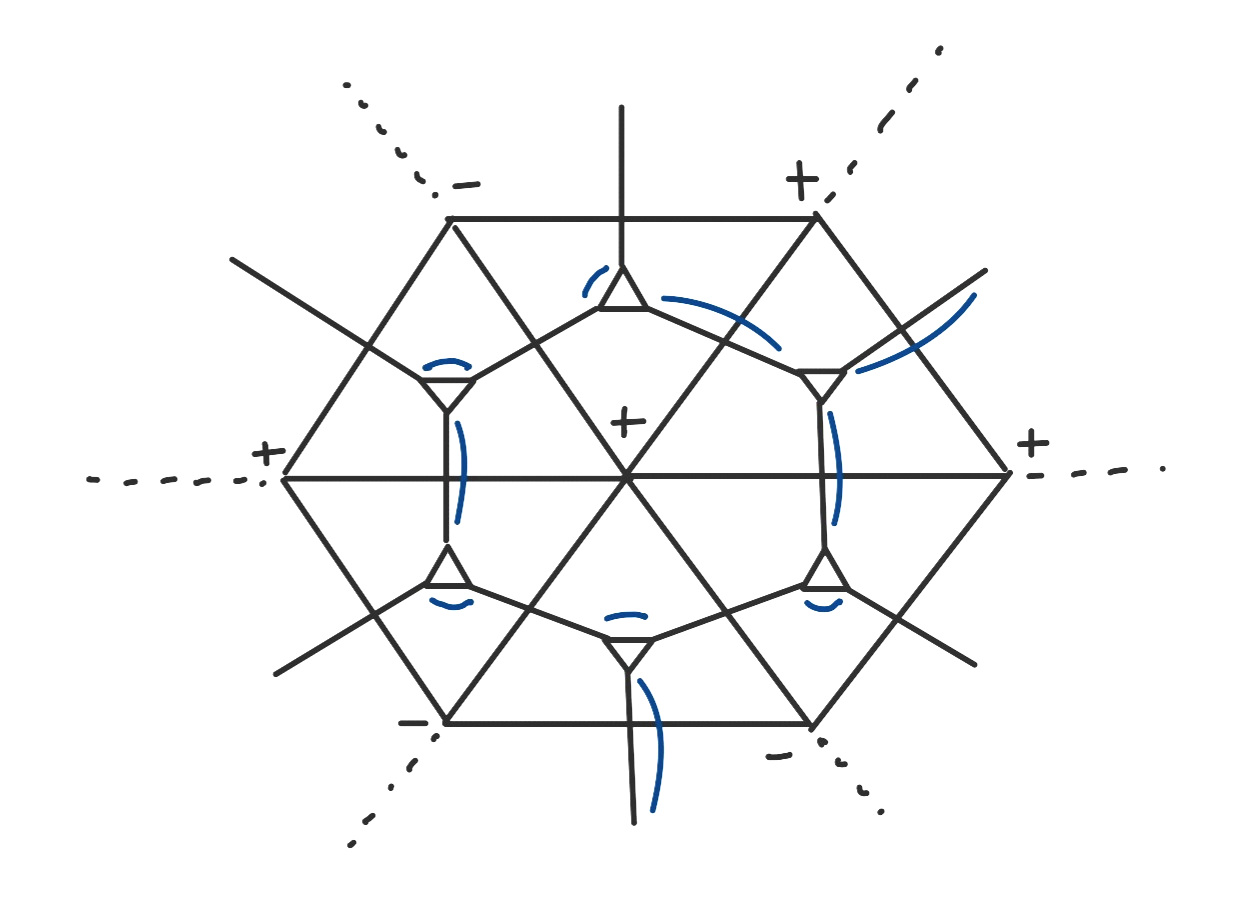
\includegraphics[width=\textwidth]{Triangular.jpg}
			\caption{Triangular}
			\label{fig:img1}
		\end{subfigure}
		\hfill
		\begin{subfigure}[b]{0.25\textwidth}
			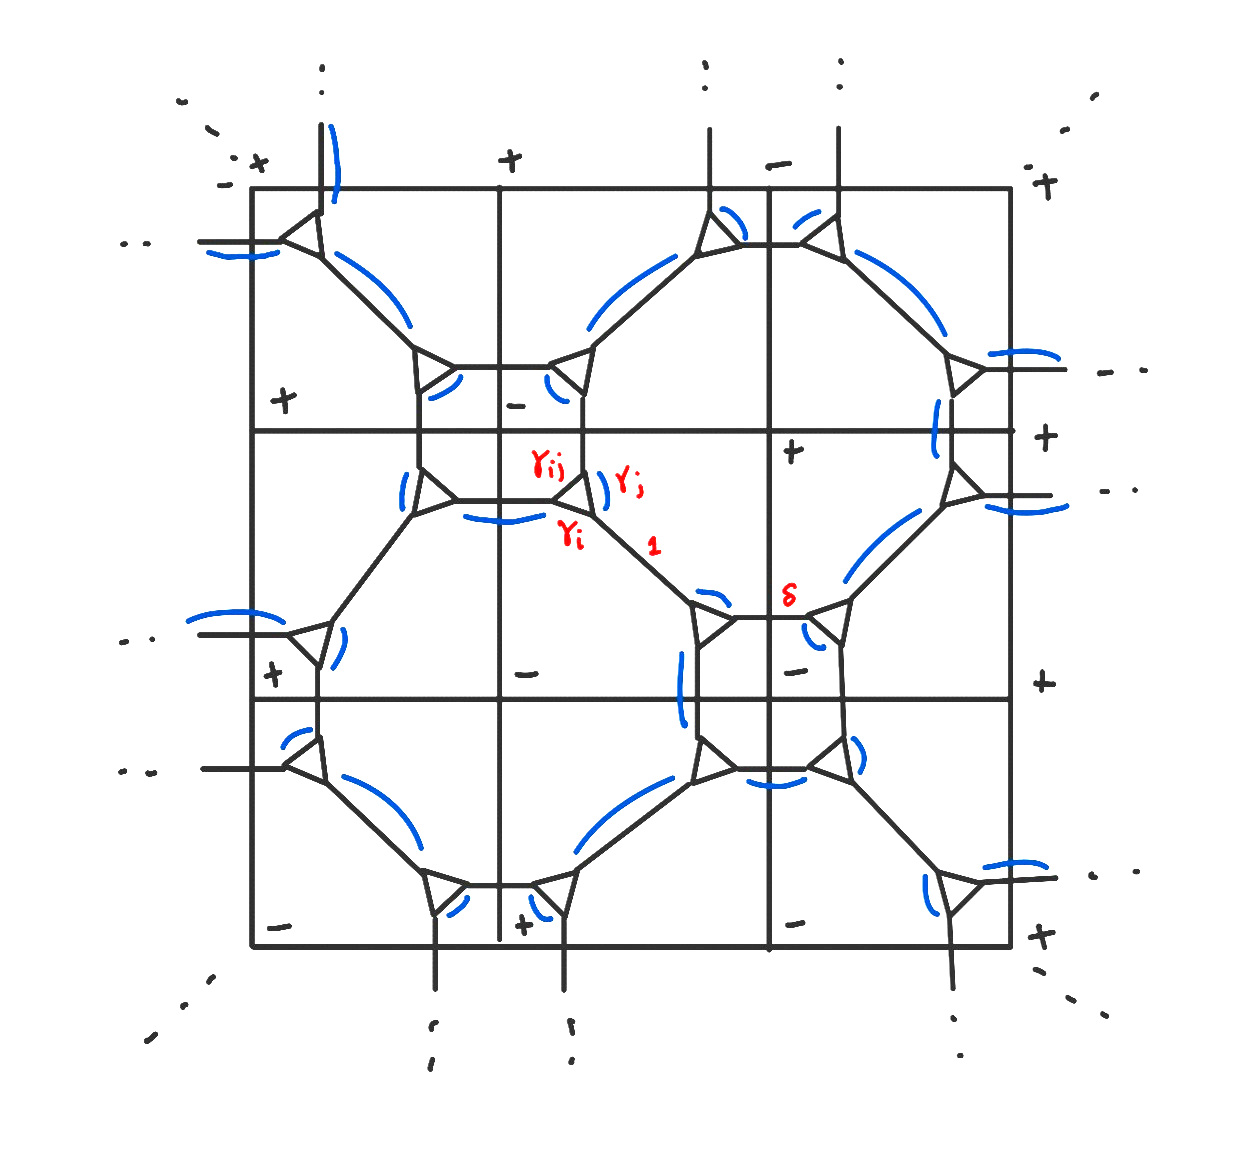
\includegraphics[width=\textwidth]{Square dimer.jpg}
			\caption{Square}
			\label{fig:img2}
		\end{subfigure}
		\hfill
		\begin{subfigure}[b]{0.25\textwidth}
			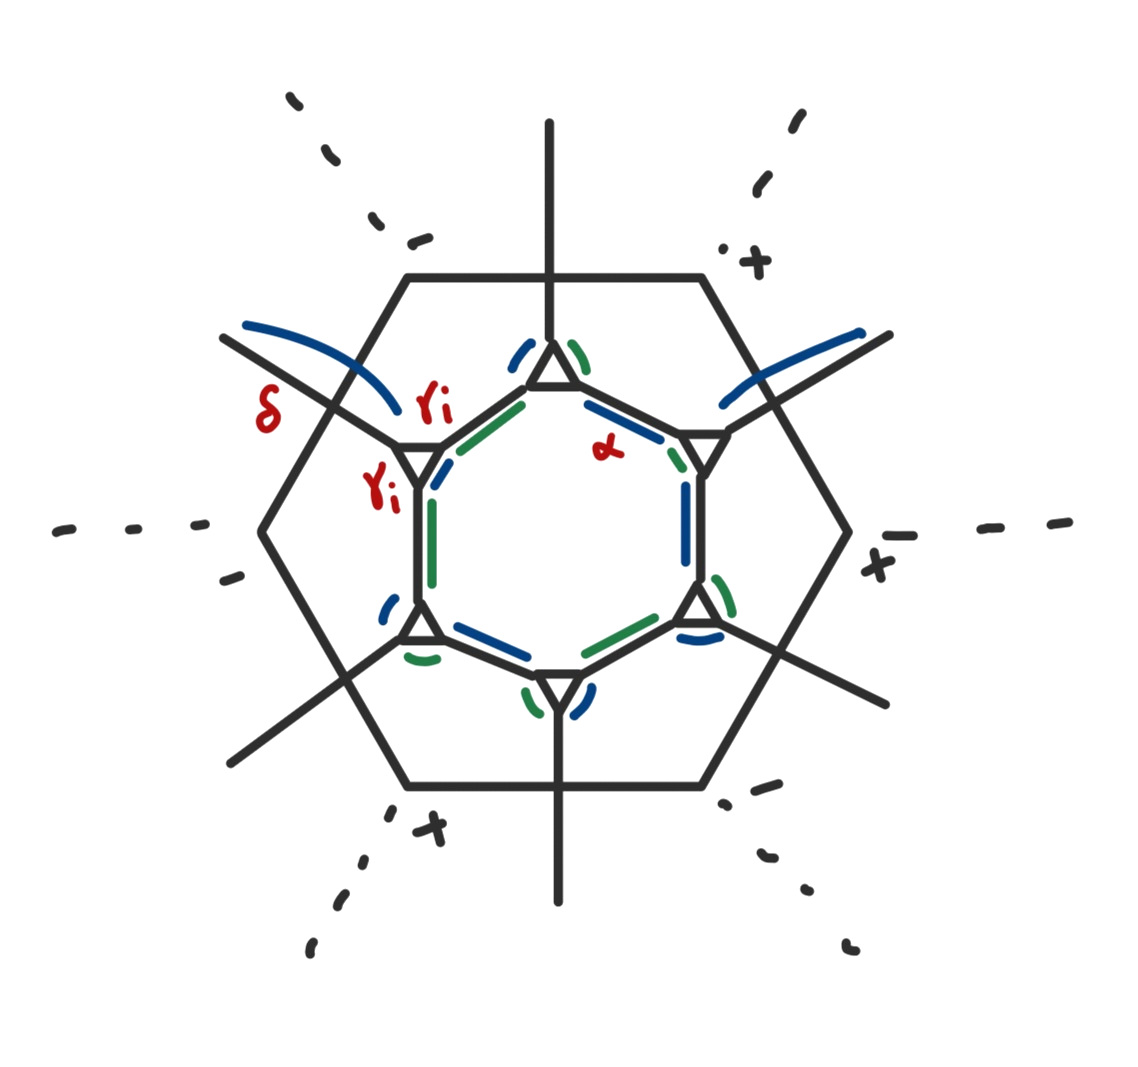
\includegraphics[width=\textwidth]{Hexagonal.jpg}
			\caption{Hexagonal}
			\label{fig:img2}
		\end{subfigure}
	\end{figure}
	
	These are the dimer mappings for spin configurations for three special cases, the first two are unique while for the hexagonal lattice, the configuration has local two-fold degeneracy which is compensated by a suitable choice of weights.  We discuss all of those details for the most general setting and show how this local constructions are consistent and map the spin configurations. \\
	
	\pagebreak
	
	\textbf{General construction with positive fugacities:} We know that a dimer model can be derived using the high-temperature expansion of the partition function. But when the interaction terms are random, i.e. if we consider a spin glass we have negative weights, as $w_e=\coth(\beta J_e)$ for an edge $e$.Though this is still correct, we want to define the corresponding dimer model in a manner such that the weights are still positive. \\
	
	\begin{center}
		\includegraphics[scale=0.25]{Configuration.jpg}\\
		\textbf{Figure-1:} Spin configuration and it's dual graph perfect matching
	\end{center}
	
	Let's put spins ($\pm$) on the vertices of a graph $(G,V)$. Now, we say an edge $e^* \in E^*$ in the dual graph $(G^*, V^*)$ is occupied by a dimer if the spins on the ends of the edge $e$ (the edge which is intersected by $e^*$) are same, otherwise this edge is not covered. We can see the spin-dimer mapping in the above picture. Any plaquette $P_x$ will have an even number of $+-$ edges because if we partition $S^1$ in blue and red regions, there will always be an even number of boundaries between these two different colours. This is what allows us to map the spin configuration exactly to the dimer coverings. Like in the picture above, say a plaquette has $n_x$ number of edges and $2m$ of them are of $+-$ type. Then there are $n_x-m$ (green or blue) dimers on the inner sides. Here, each spin configuration is mapped to two locally conjugate dimer coverings. Say, all the inner sides of the dual decorated graph in $P_x$ have weights $\alpha_x$, then we have $\alpha_x=2^{-\frac{1}{n_x}}$ to compensate for one-to-two mappings. Also we have, $\delta_e=e^{\beta J_e}$. Now, out of $n_x$ if $2m$ edges are of $+-$ types, then we have $\gamma^{(0)}_e=e^{-\beta\frac{J_e}{2}}$. However, because of the one-two mapping in local plaquettes, we have a factor $2\alpha_x^{n_x-m}=2^{\frac{m}{n_x}}$ in plaquette $P_x$ if this has $2m$ number of $+-$ edges and so $\gamma_e(x) \rightarrow \gamma_e(x)\sqrt{\alpha_x}=e^{-\beta \frac{J_e}{2}}2^{-\frac{1}{2n_x}}$, here $x$ stands for plaquette $P_x$. $J>0$ is ferromagnetic and $J<0$ is anti-ferromagnetic.\\
	
	
	So, all the weights are local, i.e. depending only on the plaquette and the corresponding edge in the original graph. To get perfect matching we need to connect the boundary spins $v^* \in \partial G^*$. So, ultimately we have $Z(\beta , \{J_e\})=2\text{Pf}[\Delta(G^*, \gamma_e, \delta_e, \alpha_e)]$. \\
	
	
	\begin{center}
		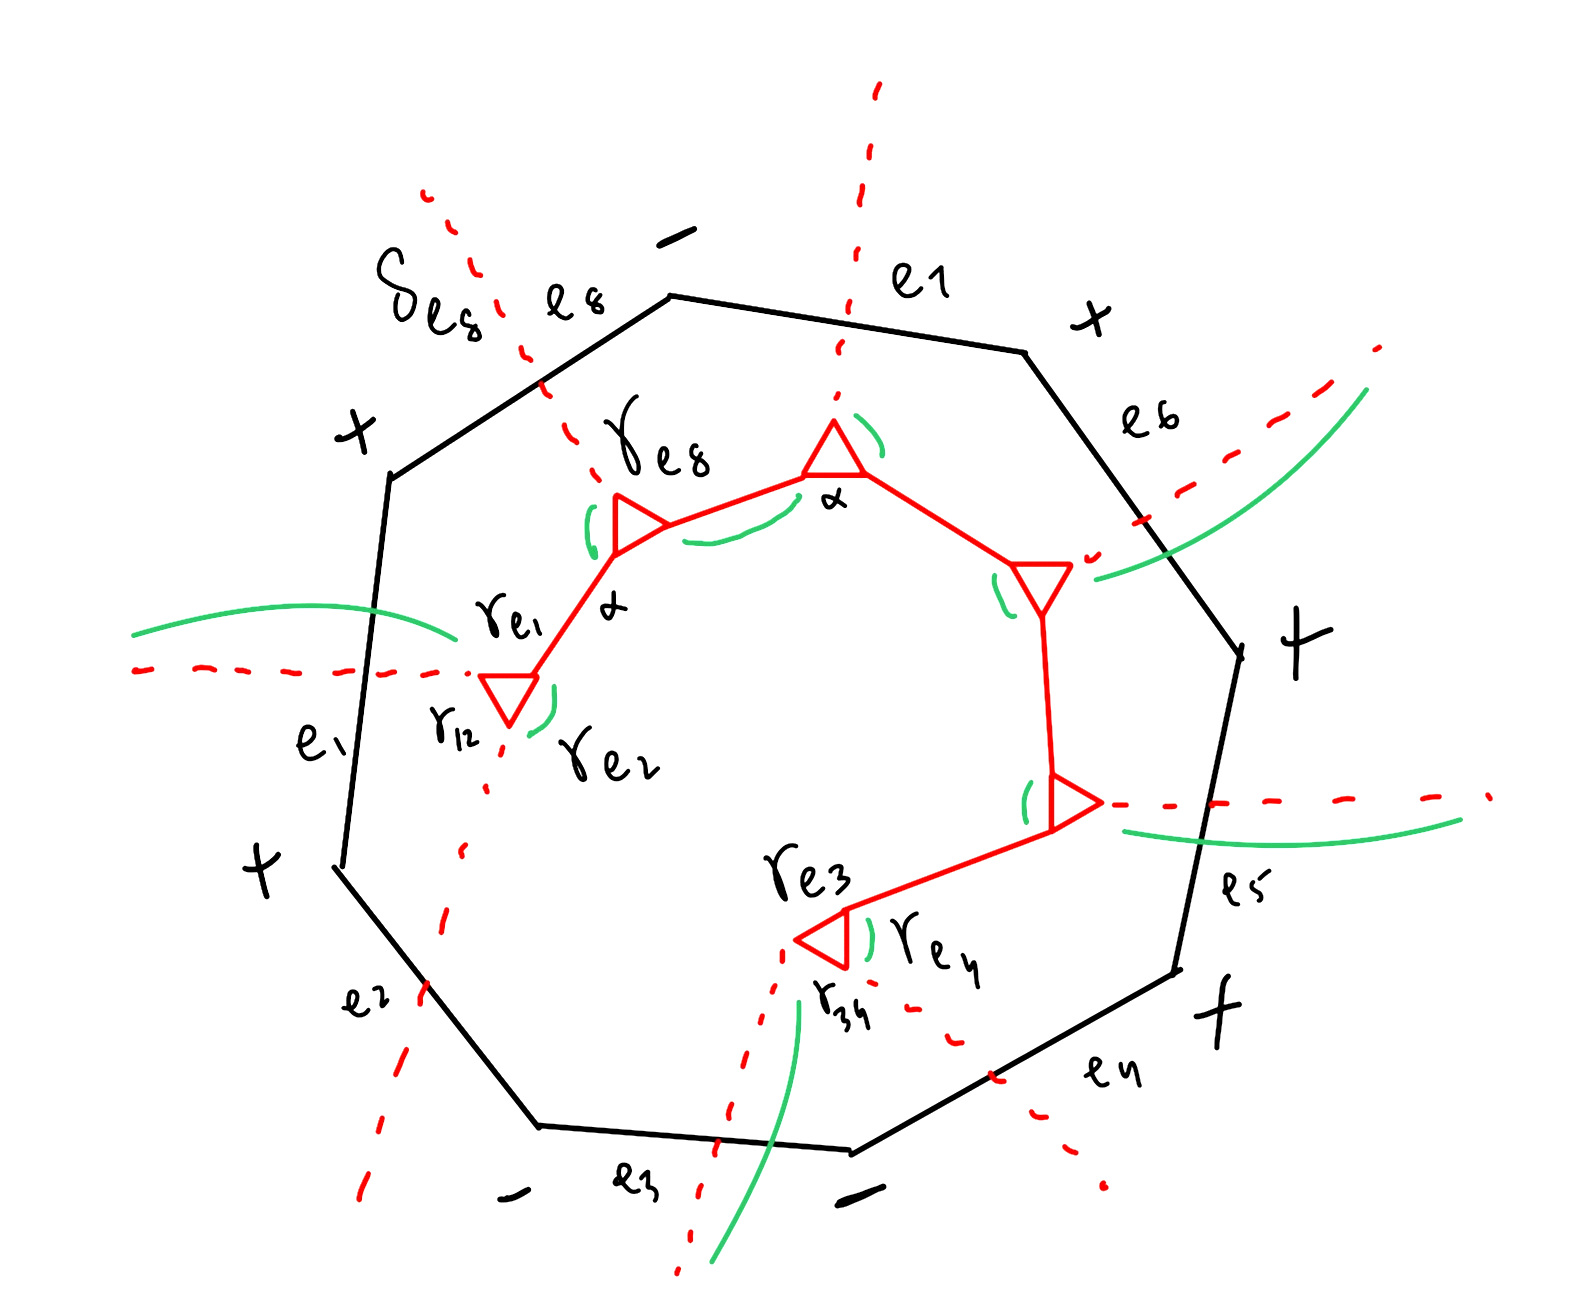
\includegraphics[scale=0.16]{Unique configuration.jpg}\\
		\textbf{Figure-2:} Unique matchings \\
	\end{center}
	
	So, far we have talked about an expander graph which results in a one-to-two mapping. However, if we take a decorated graph like that shown in the figure we will have a one-to-one mapping, even though this graph looks less symmetric. In this case, in a plaquette $P_x$ of $n_x$ edges, we have $n_x-2$ decorated triangular sites, which are precisely what we use most for the triangular and square lattices shown in Figure 3. In the case of unique matching in the above figure, we have $\gamma_{12}=\gamma_1\gamma_2$ and the same for $3,4$, i.e. the triangles at the end.
	
	\begin{center}
		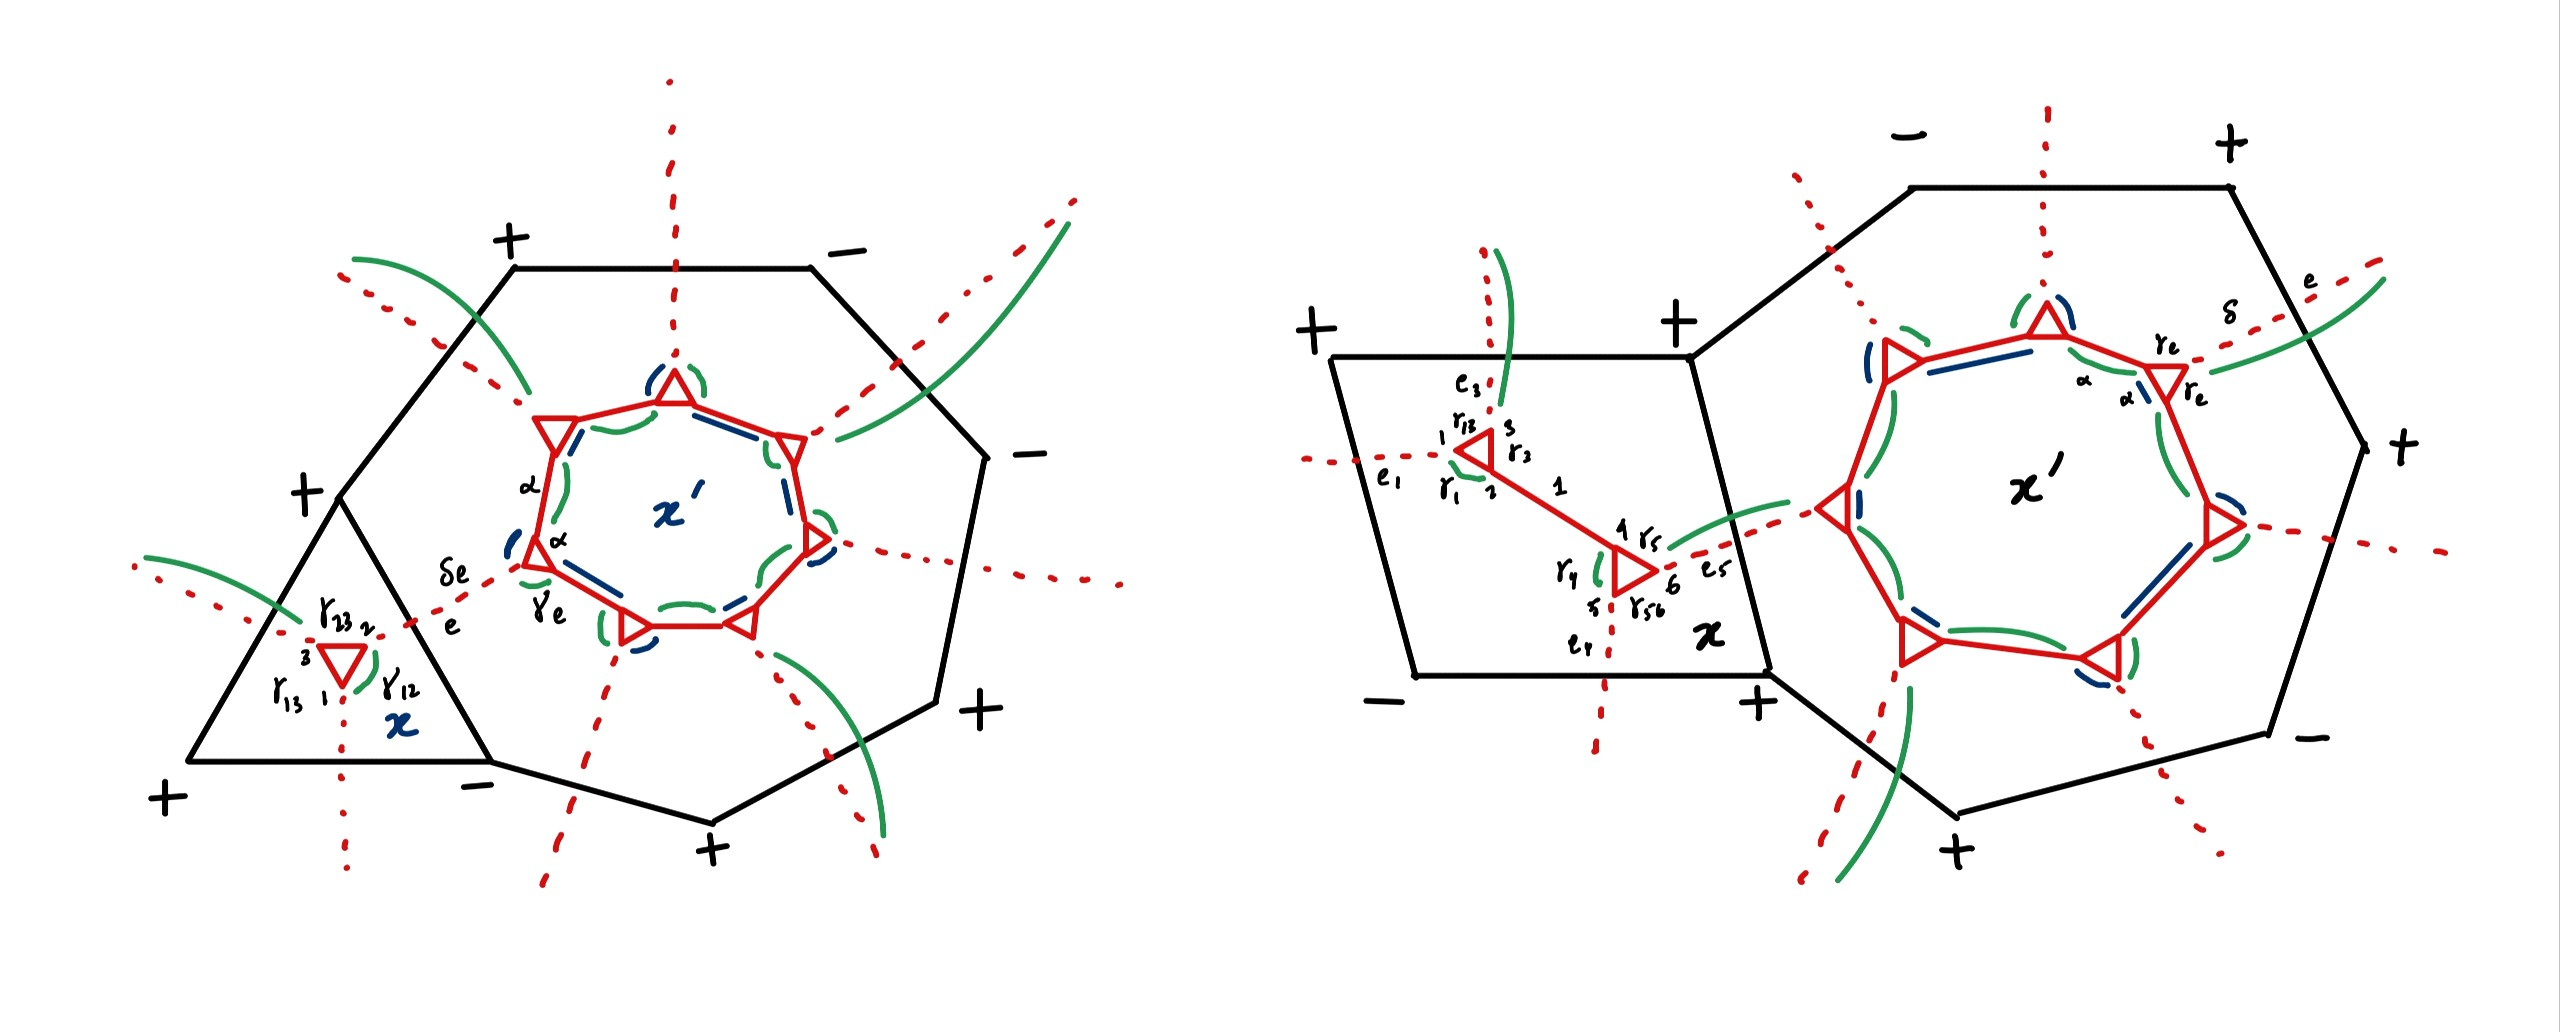
\includegraphics[scale=0.2]{Two configurations.jpg} \\
		\textbf{Figure-3:} Matchings with triangle and square plaquettes
	\end{center}
	
	These figures show the configuration where a triangle and a square are beside general polygons and these triangles and squares have the above-mentioned 'unique' decoration (that is they have one-to-one mappings). The weights on the general polygon are exactly the same as before, but the weights on the triangle in the triangular graph are modified as $\gamma_{ij}=\gamma_{i}\gamma_{j}$ where $i,j$ are two adjacent edges and $\gamma_{ij}$ are the side in between $i$ and $j$ on the decorating triangle. Similar as before, $\gamma_i=e^{-\beta \frac{J_i}{2}}$.\\
	
	A key property that makes this mapping possible is that there is always an even number of boundaries between red and blue regions on $S^1$ which is not true when there are more than two colours (spins) failing us to make a construction for $q>2$-potts models. \\
	
	$\textbf{Dimer representation for magnetization:}$ The general construction was done for zero magnetic field. In all the representations in the literature, a complete dimer representation is done for zero magnetic fields because a magnetic field breaks the $\mathbb Z_2$ symmetry. But we have mentioned that the boundary of the dual graph $G^*$ needs to be connected to get perfect matchings always and this gives a one-to-two mapping. Here we show that we can exploit this to get a dimer representation when a magnetic field acts on the boundary spins. \\
	
	\begin{figure}[h]
		\centering
		\begin{subfigure}[b]{0.43\textwidth}
			\includegraphics[width=\textwidth]{Boundary field.jpg}
			\caption{Boundary field dimer map}
			\label{fig:img1}
		\end{subfigure}
		\hfill
		\begin{subfigure}[b]{0.4\textwidth}
			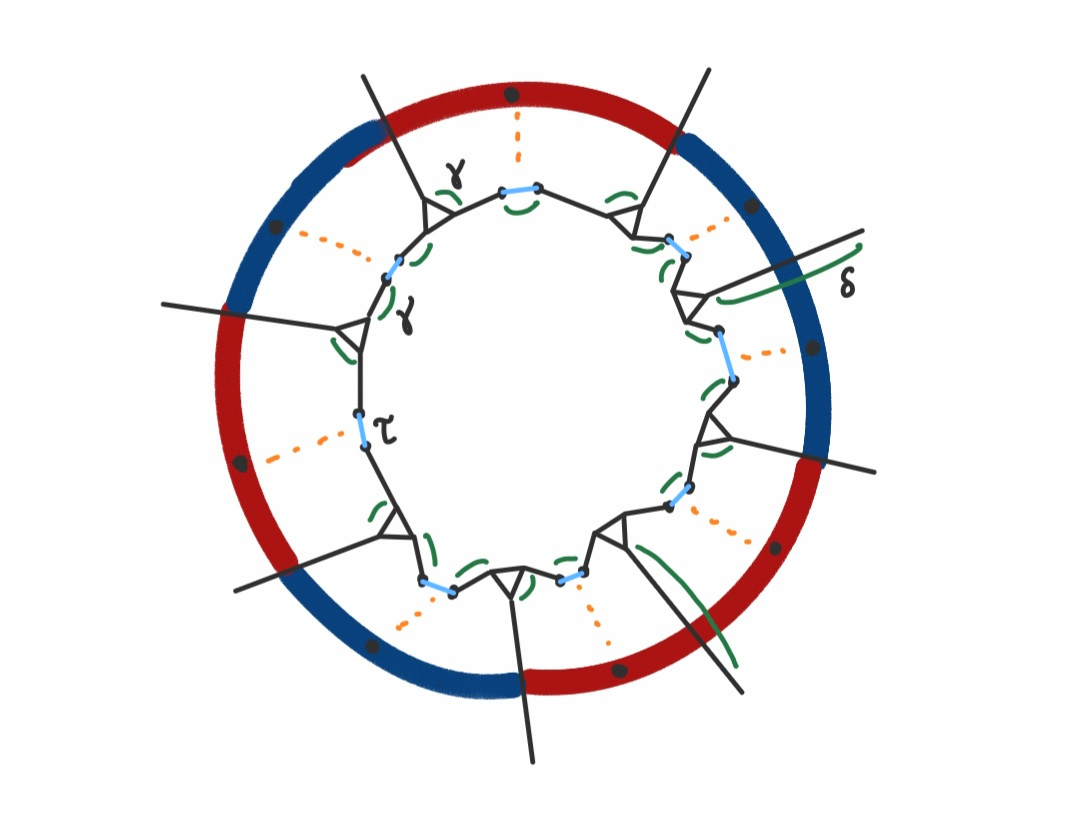
\includegraphics[width=\textwidth]{Plaquette field.jpg}
			\caption{Plaquette field dimer map}
			\label{fig:img2}
		\end{subfigure}
	\end{figure}
	
	
	We put loops (shown in orange) on each site (shown by black dots) of the boundary of $G$. Here we have taken a graph $G$, such that its boundary is smooth, i.e. we can construct the whole graph by adding plaquettes. Hence, $\partial G \cong S^1$, so its negative (shown in red) and positive (shown in blue) spins will have an even number of boundaries. \\
	
	The Hamiltonian, in the presence of a magnetic field in the boundary, is, $H=-\sum_{i,j} J_{i,j}A^{(G)}_{i,j}s_is_j-\sum_{i \in \partial G} h_i s_i $, where $A$ is the adjacency matrix for the graph. To morph this into dimer language we add virtual loops (shown in orange). In the dual graph, each of these virtual loops will enclose a pair of points connected by edges shown in sky-blue, the weights of which are $\tau_s$ where $s$ is the site. The edges that come out of the loops are labeled as $\eta_s$. If two $\gamma$ dimers on the boundaries of a region face towards each other, we colour that region with red, i.e. all the spins in that region are $-$. Hence, all the dimers (of the boundary) inside that region are on the edges inside the loops. So, we set $\tau_s=e^{-\beta h}\alpha_x$, which gives the Boltzmann weight of a negative spin in the magnetic field $h$ which is oriented in $+$ direction. As the $\eta$ edges (two legs for each site)  correspond to the blue region, we set $\eta_s=e^{\beta \frac{h}{2}}\sqrt{\alpha_x}$. This construction uniquely maps the spin configurations of the boundary sites, and because the boundary spins can be identified, every spin configuration of $G$ can be. So, $Z[\beta, J_e, h_s| s\in \partial G]=\text{Pf}[\Delta_{\text{loop}}(\beta, \gamma_e, \alpha_e, \delta_e ,\tau_s, \eta_s)]$.\\
	
	
	Using this double degeneracy we can only get dimer representation for magnetic field applied to only one plaquette or just the boundary. To get $m_{+}$ magnetization (i.e. when all the sites of boundaries are fixed to $+$) we need to have directed magnetic field on the boundary and one plaquette, which is not possible in this manner. If we put magnetic field on only one plaquette in the bulk, translational invariance breaks preventing us to get an exact expression for finite magnetic field, though we can have perturbative approximation. Instead if we put magentic field on one plaquette along some direction and put random binary fields on all other plaquettes, we get an exact avergaed partition function. We discuss this in detail in the section below. \\ 
	
	\textbf{Exact solution for plaquette Random Field Ising Model:} Owing to the above construction, we give the exact solution to the averaged partition function in the presence of a fixed magnetic field $h$ to a plaquette and $\pm h$ magnetic field on all other plaquettes. If instead, we apply a magnetic field to only one plaquette and zero to the other, the translational symmetry and we can not find an exact solution. However applying an up-down magnetic field to each plaquette, we restore this symmetry. The exact dimer mapping gives the following unit configuration which is in all the plaquettes. This unit configuration comes from the general construction shown in the previous diagram.
	
	\begin{figure}[h]
		\centering
		\begin{subfigure}[b]{0.3\textwidth}
			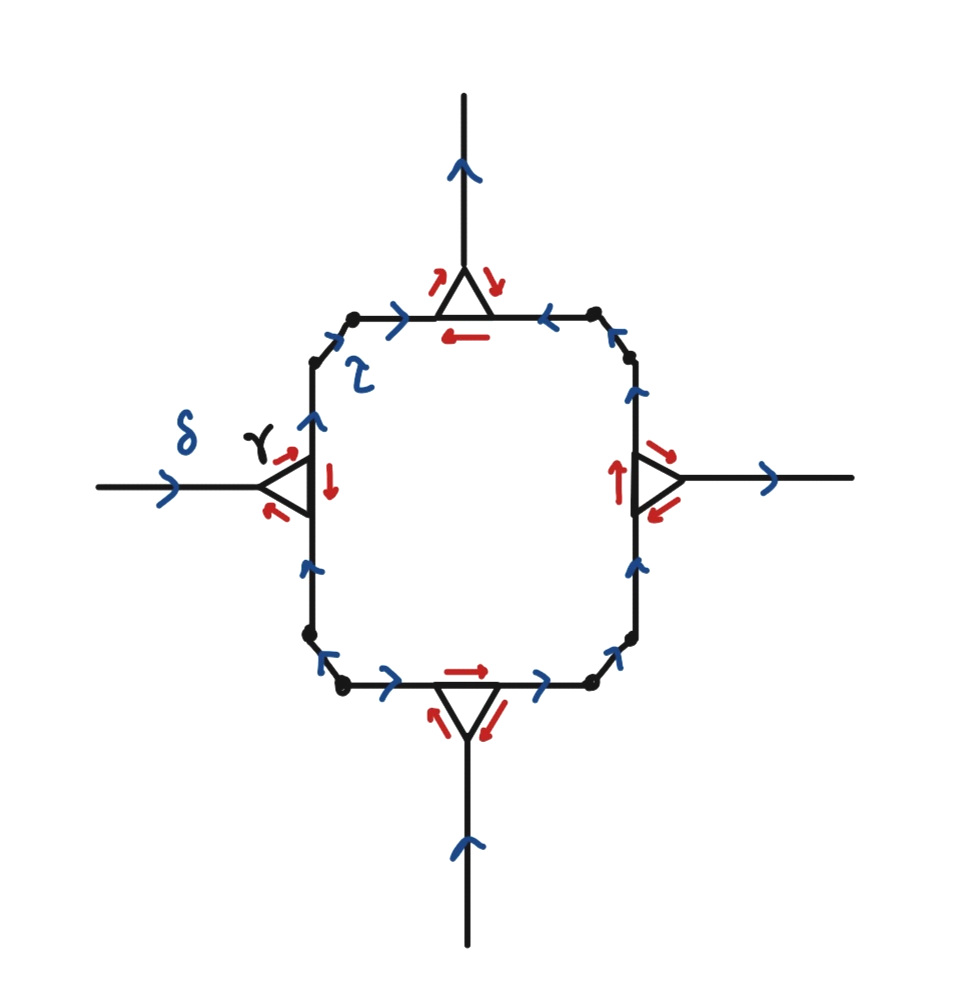
\includegraphics[width=\textwidth]{Square.jpg}
			\caption{Unit configuration}
			\label{fig:img1}
		\end{subfigure}
		\hfill
		\begin{subfigure}[b]{0.5\textwidth}
			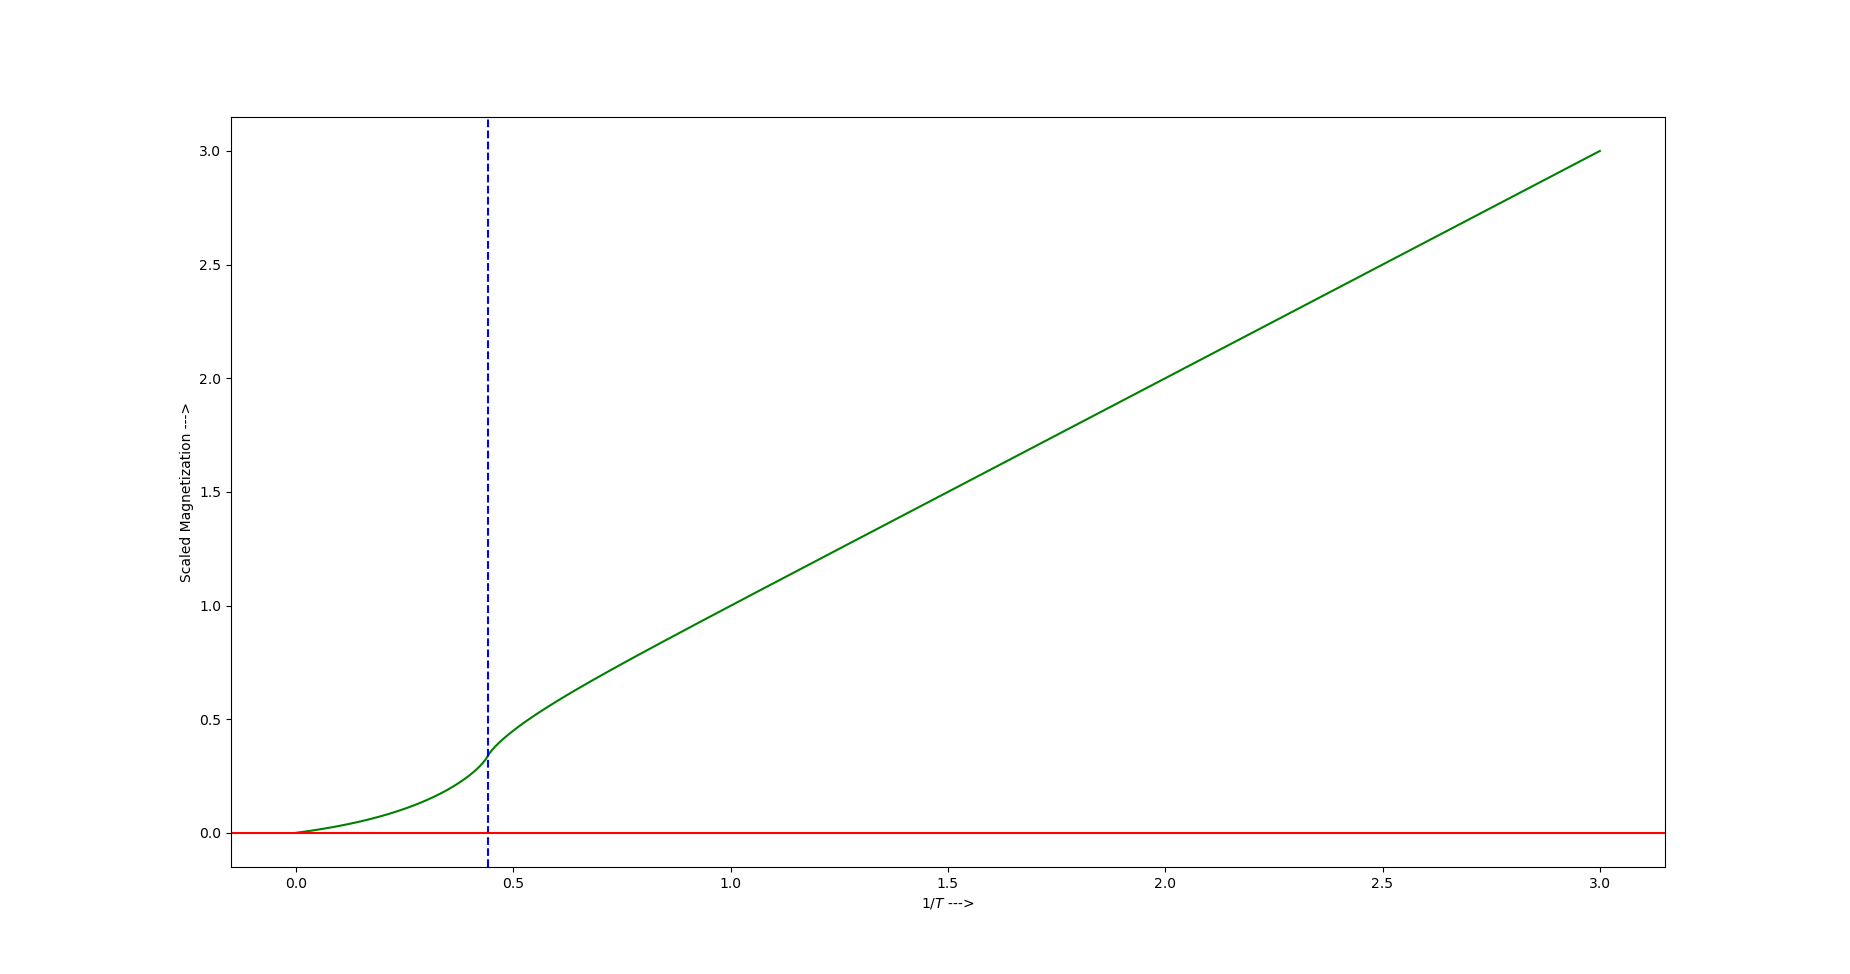
\includegraphics[width=\textwidth]{Scaled Magnetization.png}
			\caption{Scaled magnetization for binary field}
			\label{fig:img2}
		\end{subfigure}
	\end{figure}
	 
	 The average partition function for this random field ising model is $\tilde Z=\frac{1}{|\Omega|}\sum_{\omega \in \Omega} Z[\omega]$. Hence, the expected magnetization is $m=\frac{1}{|\Omega|}\sum_{\omega} m(\omega) $$= \lim \limits_{h \to 0^+}\frac{1}{\beta |\Omega|} \sum_{\omega} \partial_h \ln Z[\omega] = \lim \limits_{h \to 0^{+}} \partial_h \ln \tilde Z$ as $Z_w=Z_0 \forall w \in \Omega$ at $h=0$. \\
	 
	 Now, $\tilde Z=\text{Pf}\Delta[\beta, J, h]$, where $\Delta$ is a  matrix for the whole lattice. 
	 This circulant matrix block diagnolizes in $20 \times 20$ matrices $A(r,s)$ which gives $\ln \tilde Z(h)=\frac{1}{8 \pi^2}\int_{0}^{2 \pi} \int_{0}^{2 \pi}d\phi_1 d\phi_2 \mathcal{D}(\phi_1,\phi_2)$, with $\mathcal D=\ln [\det[A(r,s)]], \phi_1=\frac{2\pi r}{m}, \phi_2=\frac{2\pi s}{n}$ in $m,n \to \infty$ limit.  Using Mathematica we find the final expression for this field averaged partition function: 
	
	\begin{align}
		\ln[\tilde Z[\beta, J, h]] &= \frac{1}{8\pi^2} \int_{0}^{2\pi} \int_{0}^{2\pi} \ln \Bigg[ \frac{1}{4} \Bigg( 8 + 4e^{-4\beta J} + 2e^{4\beta J} + 2e^{4\beta J}\cosh(2\beta h) \nonumber \\
		&\qquad - 8(\cos(\phi_1) + \cos(\phi_2))[e^{2\beta J}\cosh(\beta h)-e^{-2\beta J}] \nonumber \\
		&\qquad -4[\cos(\phi_1-\phi_2)+ \cos(\phi_1+\phi_2)](\cosh(\beta h)-1) \nonumber
		\Bigg) \Bigg] d\phi_1 d\phi_2
	\end{align} 
	
	Hence, $\chi_0=\lim \limits_{h \to 0^+} \frac{m(h)}{h}=\lim \limits_{h \to 0^+} \frac{1}{\beta h}\partial_h \ln Z_h = \lim \limits_{h \to 0^+}  \frac{1}{h|\Omega|}\sum_{\omega \in \Omega} \langle \sum_{i} \omega_i \sigma_i \rangle_{+}$ (where $\omega$ are all $\pm$ configurations) is shown in the figure above. We note that the phase transition of this modified random field averaged magnetization is no longer of second order, but we can see that $\mathcal D(\beta, 0,0)=0$ at $\beta=\frac{1}{T_c}$. This random field magnetization scales with $h$ near $0$. We can see that for $h=0$, this is exactly the Onsager solution.\\ 
	
	
	Now, $\mathbb E[m^2]=\frac{1}{|\Omega|}\sum_{\omega} m^2_{\omega} =\lim \limits_{h \to 0^+} \frac{1}{\beta^2}[\partial^2_h \ln \tilde Z+(\chi_0 h)^2] = \lim \limits_{h \to 0^+} \frac{1}{\beta^2}[\partial^2_h \ln \tilde Z]$. \\
	
	\begin{center}
		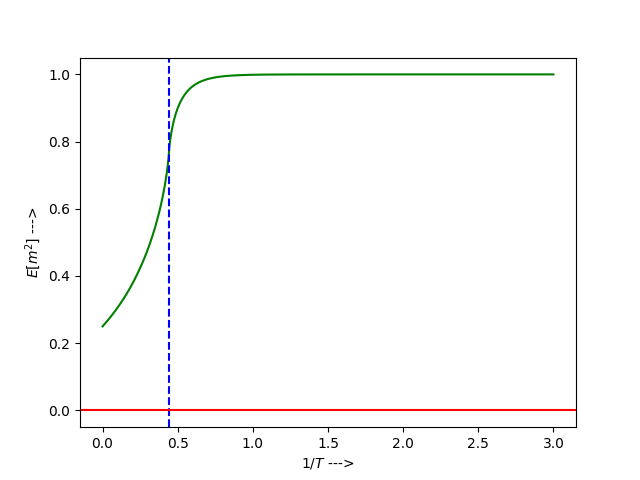
\includegraphics[scale=0.2]{Susceptibility.png}\\
	\textbf{Figure-5:} $\mathbb E[m^2]$ for Plaquette RFIM\\
	\end{center} 
	
	Though there are perturbative methods to find magnetization due to Yang and others, an exact solution for the partition function of the $2$-D Ising model in the presence of an external magnetic field is still an unsolved problem. The $\bar m^2$ in this case will be zero for $T\leq T_c$ and non-zero for $T >T_c$. On the other hand, if we consider a random field on each site, we get $\chi_0=1$ for all temperatures, $\bar m^2$ is always $1$, which is trivial. The above solution considers random fields on the plaquettes, which is a step towards the complete solution as this captures the global symmetry breaking to `a plaquette's' extent.We can see that in the above figure as this is in between the above two cases. To get even closer behavior, we may take multiple plaquettes and put field (so the modified construction) into a single plaquette and tile up the whole space with this, this recurrently will show a sharp phase transition of the magnetization.\\
	
	
	\textbf{Note on correlation:} As correlation is related to a path in the high-temperature expansion, this dual description can not find the correlation function with a simple modification. In the original Fisher construction, we can add three extra nodes around the decorating triangles at points $x_1,x_2,...$ and implement the Kasteleyn orientation on this modified graph to obtain $n$-point correlation $\langle \sigma_{x_1}\sigma_{x_2}....\sigma_{x_n} \rangle$.\\
	
	We can write $\langle \sigma_x \sigma_y\rangle=\frac{1}{Z}[Z[\sigma| \sigma_x=\sigma_y]-Z[\sigma| \sigma_x=-\sigma_y]]$, where $Z[\sigma| \sigma_x=\pm \sigma_y]=\lim \limits_{J^* \to \infty} e^{\mp\beta J^*}\sum_{\sigma} e^{-\beta H(\sigma)\pm\beta J^*\sigma_x\sigma_y}$. But we can connect $x,y$ with an edge on the plane if they are on the boundary or there is an open passage to allow such a path. We can see that this argument comes directly from the previous argument, i.e. the correlation can be found only for $x,y$ which are on the boundary or are in the same plaquette because we can put magnetic field only on the plaquettes or the boundary, which is itself a plaquette enclosing $M/PG$, where $M$ is manifold in which the planar graph $G$ lies and $PG$ is part of $M$ that the graph $G$ encloses. \\
	
	\vspace{1 cm}
	
	\textbf{Spin glasses and lattice worms:} Each perfect matching $M$ corresponds to a spin configuration. Going from one matching $M_1$ to another matching $M_2$ means a change in spin configuration. The cluster size that has changed (entropy change) depends on $|M_1\Delta M_2|$. We can go from $M_1$ to $M_2$ by performing worm dynamics, the size of the worm will indicate the size of the cluster change. \\
	
	A possible advantage of using worm dynamics for spin glass: In the spin glass problem if we flip one spin, the change in energy may be very high, which hinders the efficiency of Monte Carlo simulation. However, in this new language, we don't flip a spin resulting in high energy cost, instead, we rotate dimers, each of which is more efficient and increases the power of Monte Carlo. \\
	
	\vspace{0.5 cm}
	
	\textbf{Worm dynamics on decorated triangular graph:} Now we perform the worm dynamics on the decorated triangular graph that we get for the dual lattice of $(3,6)$ with arm-chair boundary. \\
	
	We perform worm dynamics on the dual graph of the hexagonal lattice. We perform a sequential operation similar to the Monte Carlo method, however, once we start the worm dynamics, we can't stop until another perfect match is there. The probability of going from $e_1 \to e_2$ is $\frac{w_{e_2}}{\sum_m w_{m}}$, where $m$ are all the other edges adjacent to $e_1$. Below we show the probability distribution of cluster size for random $\pm J$ spin for different temperatures.\\
	
	
	\begin{figure}[h]
		\centering
		\begin{subfigure}[b]{0.4\textwidth}
			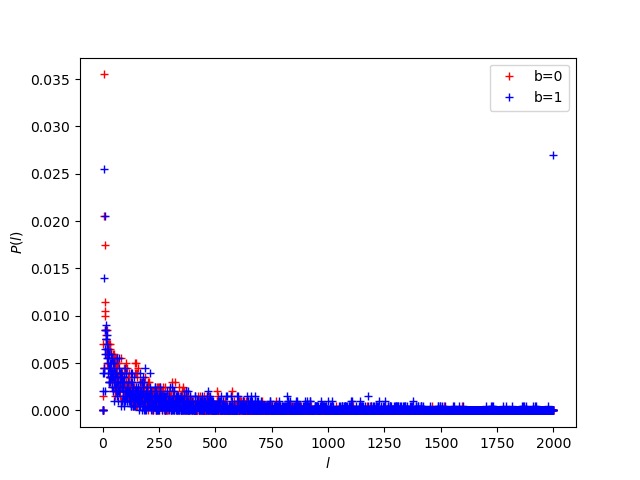
\includegraphics[width=\textwidth]{Spin glass cluster size dist 3.png}
			\caption{Cluster size distribution}
			\label{fig:img1}
		\end{subfigure}
		\hfill
		\begin{subfigure}[b]{0.5\textwidth}
			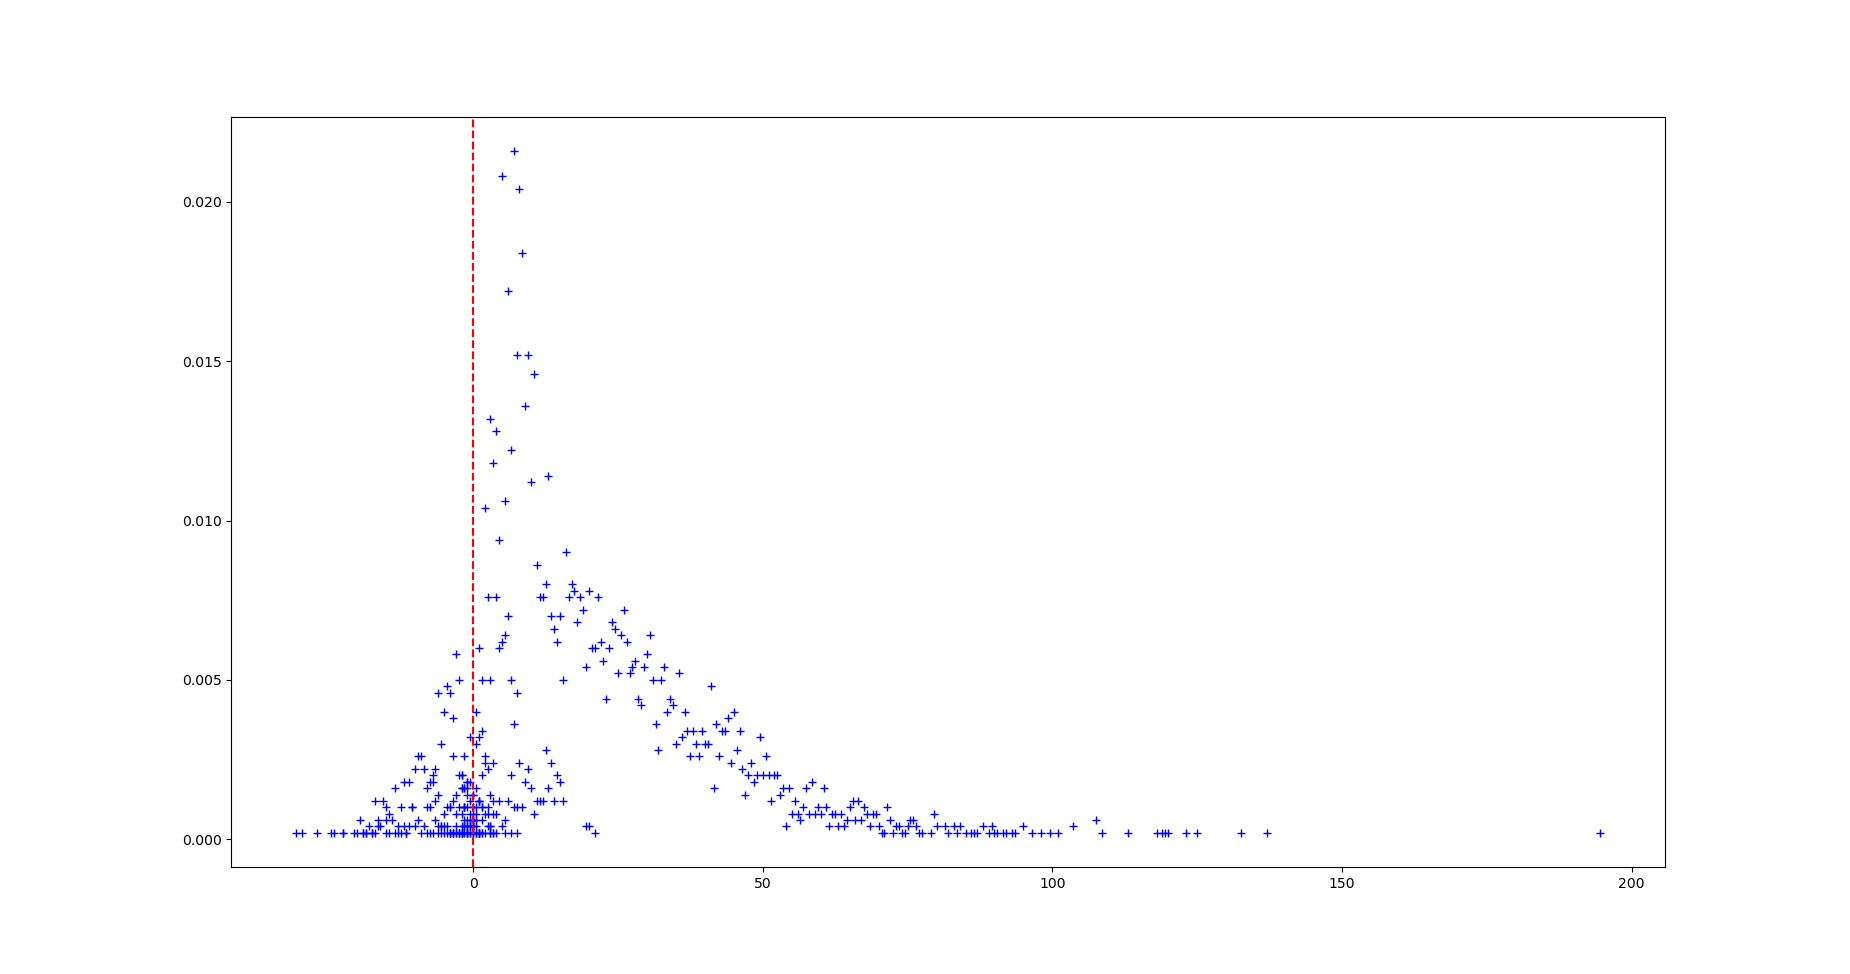
\includegraphics[width=\textwidth]{Energy distribution for spin glass 2.png}
			\caption{Single cluster energy distribution}
			\label{fig:img2}
		\end{subfigure}
	\end{figure}
	
	This worm dynamics give us the distribution of cluster size of the original spin glass problem, with the caveat that we get only one flipped connected cluster which is surrounded by the worm. But this shows us the local randomness of near arbitrary points. To compare with Ferromagnetic case we show the energy distribution for this case here as well. For the former case, the randomness is manifest in the distribution and for Ferromagnetic case we see a clear bell shaped pattern. 
\begin{center}
	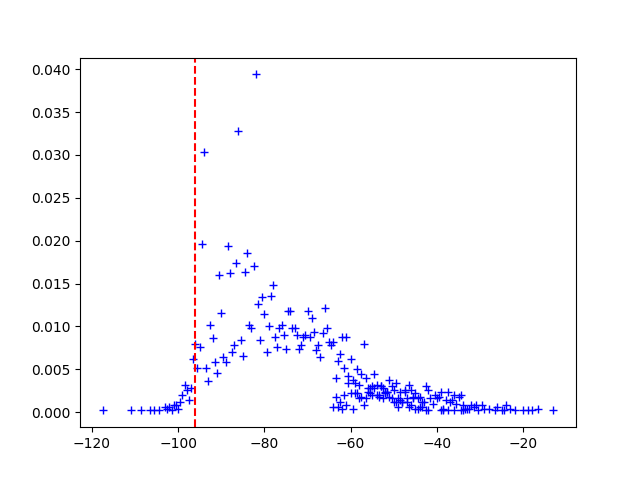
\includegraphics[scale=0.5]{Ferromagnet Energy Distribution.png}
\end{center}
	 To get the actual picture we should randomly pick the initial pivot point, perform worm dynamics and when it stops we pick a new pivot point outside of this already flipped region and perform the same worm dynamics. 
	
	
\end{document}